	\section{Transferlernen und 'Greifer beladen'-Klassifikation}
	\label{sec:TLGrappleLoaded}
	Um einen Transfer auf neue Aufgaben durchführen zu können wurde ein neues Werkzeug TransferTaskFocusAE erstellt. Dieses Werkzeug basiert auf dem TaskFocusAE und ersetzt den fokusierenden Task.
	\subsection{Werkzeug: TaskTransferOnAutoencoder}
	\label{sec:TransferSecondCriterionAutoenocder}		
	Ein TransferSecondCriterionAutoenocder basiert auf einem SCAE. Das zweite Kriterium wird durch ein neues Kriterium ersetzt. Zum Beispiel kann ein SCAE eine Objektkennung durchführen. Bei einem TransferSecondCriterionAutoenocder wird die Objektkennung durch eines Klassifizierungsaufgabe ersetzt. Die Architektur und die Gewichte des Autoencoders werden weiterverwendet. Abbildung \ref{img:SchemaTSCAE} zeigt den Aufbau des TSCAE.
	\begin{figure}[h]
		\centering
		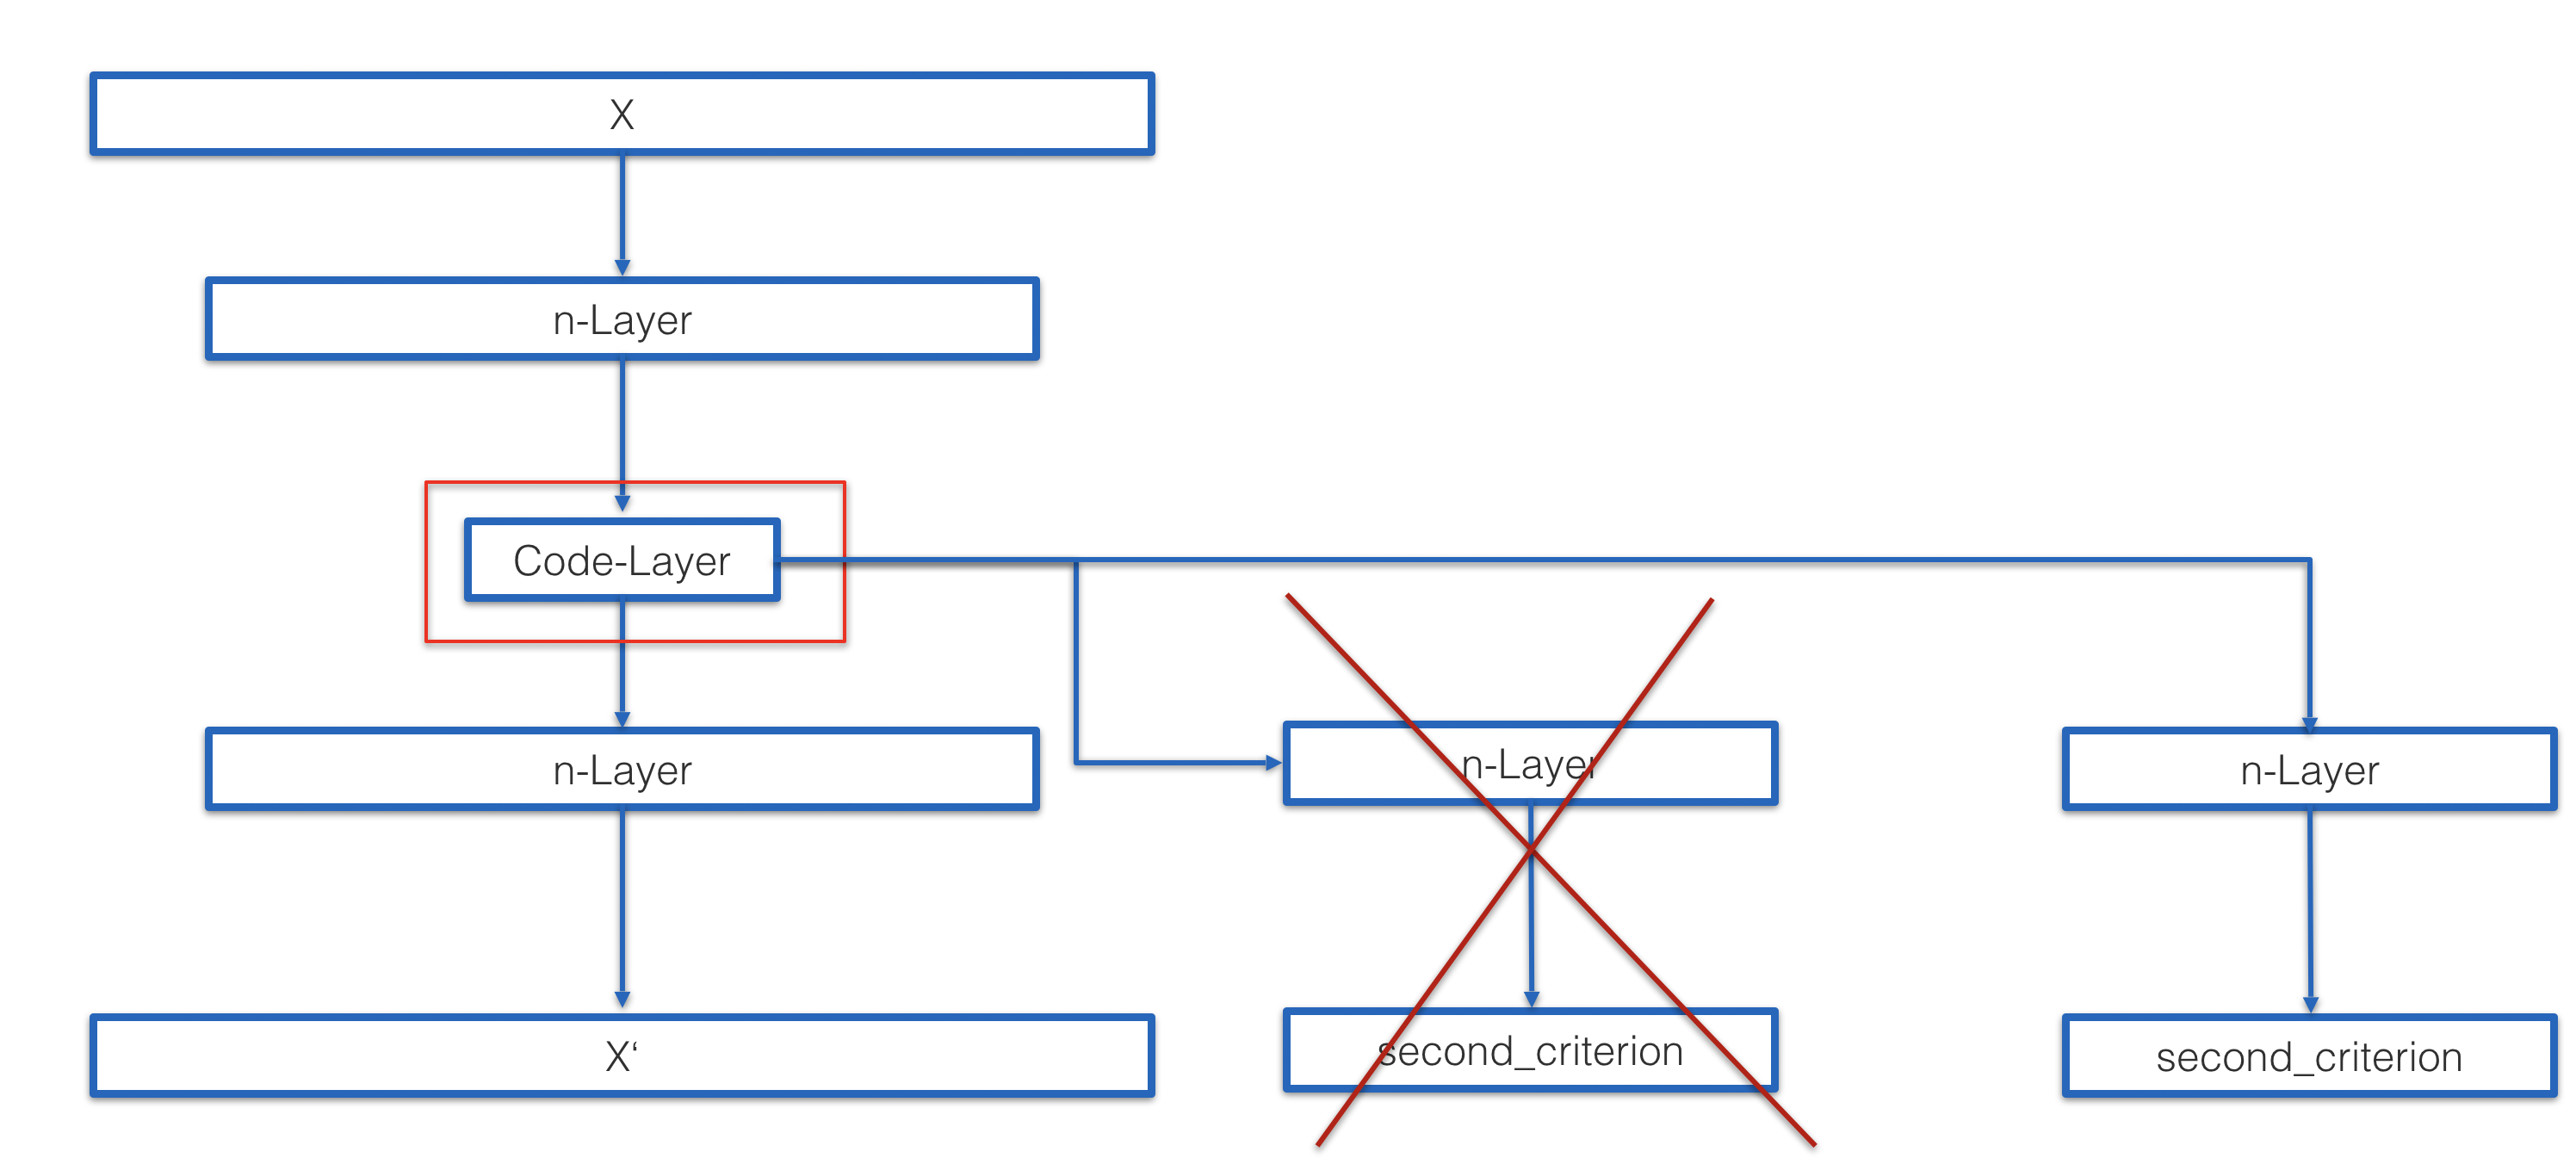
\includegraphics[width=0.5\textwidth, center]{bilder/Schema_Autoencoders/Schema_TSCAE.png}
		\caption[Schema TransferSecondCriterionAutoenocder]{Schema TransferSecondCriterionAutoenocder}
		\label{img:SchemaTSCAE}
	\end{figure}  
	Im Klassendiagramm \ref{img:KlassendiagrammTransferSecondCriterionAutoenocder} für den TSCAE ist zu sehen. Das Besondere ist, dass ein SCAE als Konstruktorargument übergeben wird. Die Einstellungen für den ConvolutionalAutoencoder werden aus diesem Model kopiert. Zusätzlich müssen nur noch die Einstellungen für das zweite Kriterium übergeben werden. Aus diesen wird das Model für das zweite Kriterium erstellt.
	Neu hinzugekommen ist, ein Parameter(freeze\_encoder\_layers) über den eingestellt werden kann, ob und welche Schichten nicht neu trainiert werden können. Es können direkt Schichten ausgewählt werden oder es kann über einen Ganzahlenwert beginnend über die erste Schicht Schichten eingefroren. Werden nur Werte für den Encoder übergeben, werden Werte für den Decoder (freeze\_decoder\_layers) daraus abgeleitet. 
	\begin{figure}[h]
		\centering
		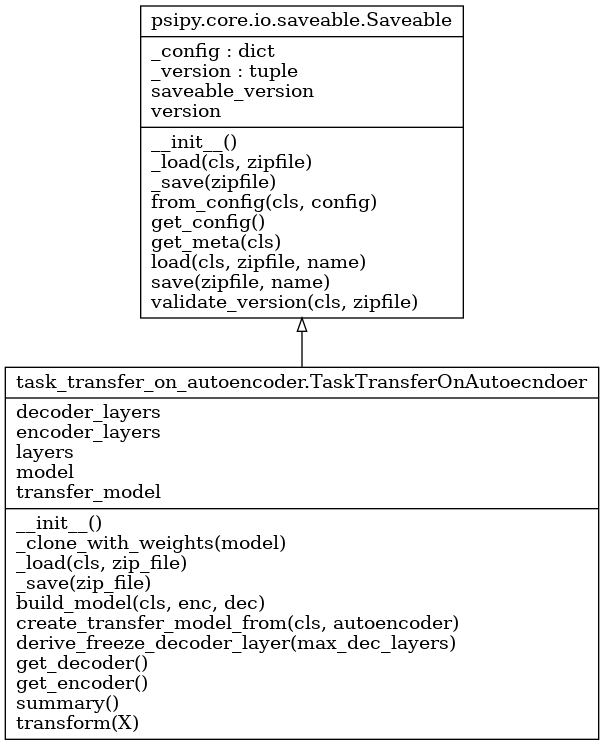
\includegraphics[width=0.5\textwidth, center]{bilder/Klassendiagramme/TTAE.png}
		\caption[Klassendiagramm TransferSecondCriterionAutoenocder]{Klassendiagramm TransferSecondCriterionAutoenocder}
		\label{img:KlassendiagrammTransferSecondCriterionAutoenocder}
	\end{figure}  
	Listing \ref{lst:BspTransferSecondCriterionAutoenocder} zeigt beispielhaft die Anwendung dieses Werkzeuges. Im Vergleich zu dem SCAE ist die Anwendung schon deutlich einfacher. Es gibt weniger Hyperparameter zum Beachten. Da das Modell auf einem trainierten SCAE basiert ist kein $pretrain(..)$ mehr notwenig. Die Methode $fit(..)$ wird auf dieselbe Weiße wie bei SCAE angewendet.	
	
	
	\begin{lstlisting}[language=python,caption=Beispiel TransferSecondCriterionAutoenocder in Python, label=lst:BspTransferSecondCriterionAutoenocder]
	tscm = TransferLearningConvolutionalSecondCriterionAutoencoder(csc_autoencoder,
	second_criterion_topology=second_criterion_topology,
	second_criterion_loss = 'binary_crossentropy',                                                                                                   
	second_criterion_hidden_layer_kwargs = {'activation': 'relu'},
	second_criterion_output_layer_kwargs = {'activation': 'sigmoid'}, 
	loss_weights=[1, 0.01],
	freeze_encoder_layers = 2
	,freeze_decoder_layers =[0,1])
	
	history = tscm.fit(
	x_train,
	{"decoder": x_train, "second_criterion": y_train}, 
	epochs=1,
	batch_size = 128,
	validation_data=(x_test,{"decoder": x_test, "second_criterion": y_test}))
	)
	\end{lstlisting}	
		
		\subsection{Ergebnis}
		In Abbildung ist das Ergebnis einen TrasnferTFAE zu sehen, es wird beinahe der selbe Score erreicht.


	\section{AutoMl und 'Greifer beladen'-Klassifikation}
	\label{sec:todo}
	Ein Hyperparameter des TransferTFAE ist die Gewichtung der Verlustfunktion. Es soll herausgefunden werden, welchen Einfluss der Hyperparameter auf die Ergebnisse hat. Da es sehr viele Möglichkeiten für die Gewichtung der Verlustfunktion gibt wird hierzu ein neues Modul erstellt. Dieses Modul greift auf den AutoMl-Ansatz der automatischen Hyperparameteroptimierung zu.
		\subsection{Werkzeug: AutoFocusTransferOnAutoencoder}
		\label{sec:AutoTransferSecondCriterionAutoenocder}
		Der AutoTransferSecondCriterionAutoenocder ist ein TransferSecondCriterionAutoenocder welcher mithilfe von HpBandSter AutoML zur Hyperparameteroptimierung einsetzt. Konkret  erbt die Klasse von hpbandster.core.worker. Zur Speicherung und Verwaltung der Hyperparameter wird auf die Klasse HyperparameterMixin zurückgegriffen. Bei der Instanziierung der Klasse werden sinnvolle Standardwerte für Hyperparameter gesetzt. Die Werte können aber später noch angepasst werden. 
		In Abbildung \ref{img:KlassendiagrammAutoTransferSecondCriterionAutoenocder}  ist das zugehörige Klassendiagramm abgebildet. 
		\begin{figure}[h]
			\centering
			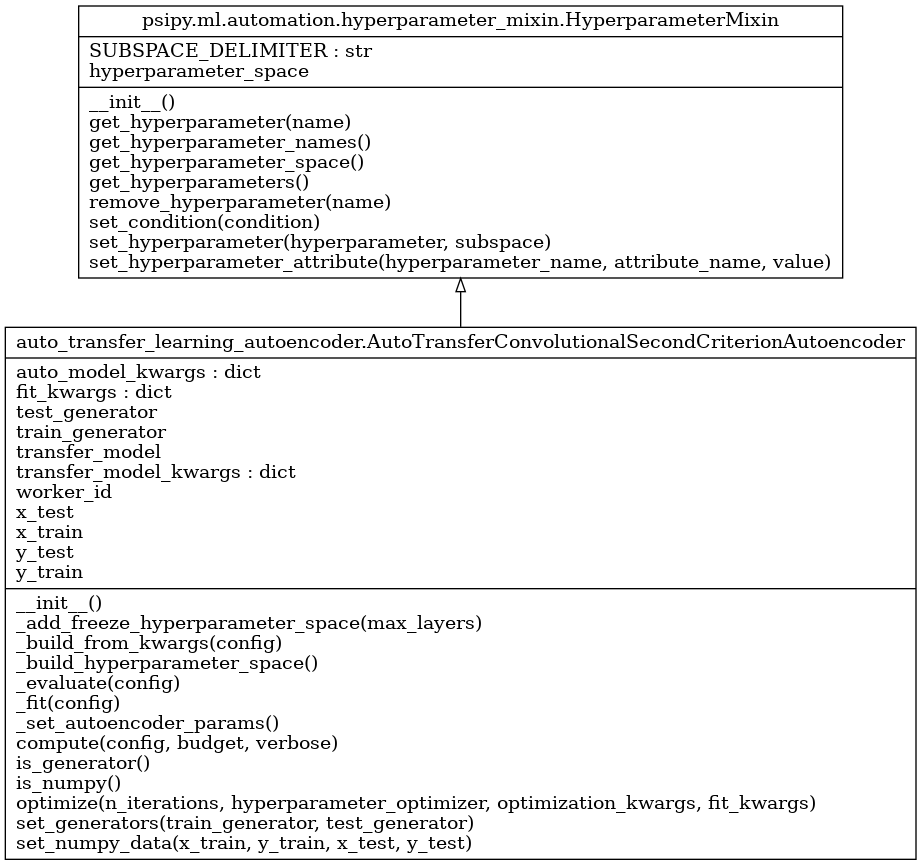
\includegraphics[width=0.5\textwidth, center]{bilder/Klassendiagramme/Klassendiagramm_AutoTLCSCAE.png}
			\caption[Klassendiagramm AutoTransferSecondCriterionAutoenocder]{Klassendiagramm AutoTransferSecondCriterionAutoenocder}
			\label{img:KlassendiagrammAutoTransferSecondCriterionAutoenocder}
		\end{figure}  
		In Listing \ref{lst:BspAutoTransferSecondCriterionAutoenocder} ist eine einfache Implementierung eines AutoTransferSecondCriterionAutoenocder dargestellt. Der Konstruktor unterscheidet sich nur an einer Stelle zum Konstruktor des TransferSecondCriterionAutoenocder. Es wird keine Instanz des SCAE übergeben, sondern ein Pfad zu einem abgespeicherten Modell eines SCAE. 
		Im Gegensatz zur bisherigen Vorgehensweise werden die Trainings und Testdaten mit der Methode $set_generators(..)$  oder $set_numpy_data(..)$ übergeben. Ziel ist es dabei die Komplexität der Methode $optimize(..)$ zu reduzieren. Durch den Aufruf von $optimize(..)$ wird der Optimierungsvorgang gestartet. Die Parameter sind dabei die Anzahl an Iterationen, die Optimierungsstrategie und ein Wörterbuch, welches zusätzliche Einstellungen für die einzelnen Optimierer enthalten kann. In jeder Iteration der Optimierung wird ein neuer TransferSecondCriterionAutoenocder erstellt und mittels der ausgewählten Hyperparameter und übergebenen Daten trainiert. 
		\begin{lstlisting}[language=python,caption=Beispiel AutoTransferSecondCriterionAutoenocder in Python, label=lst:BspAutoTransferSecondCriterionAutoenocder]
		tscm = AutoTransferConvolutionalSecondCriterionAutoencoder(max_deep_freeze=2,
		path_to_model = path_to_base_model,            
		second_criterion_topology=second_criterion_topology,
		second_criterion_loss = 'categorical_crossentropy',                                                                                                   
		second_criterion_hidden_layer_kwargs = {'activation': 'relu'},
		second_criterion_output_layer_kwargs = {'activation': 'softmax'},
		second_criterion_metrics = {'second_criterion':'accuracy'}
		)
		
		tscm.set_generators(train_datagenerator,test_datagenerator)
		
		
		best_config, history = tscm.optimize(3
		,'RandomSearch'
		,optimization_kwargs = optimization_kwargs)
		\end{lstlisting}
		Das Werkzeug unterstützt derzeit die Optimierer, Randomsearch, Hyperband und BOHB.	In Tabelle \ref{table:HyperparparameterAutoML} sind die Hyperaparameter und ihre mögliche Werte dargestellt.
		\begin{table}[ht]
			\centering
			\begin{tabularx}{\textwidth}{lll}
				\textbf{Hyperparameter} & \textbf{Werte}  & \textbf{Datentyp} 					 	\\
				\textbf{Optimierer}   & 	Adam, sgd, rmsprop		&	Kategorial			\\
				\textbf{Batch\_size}  &  32 - 1024					 &	Ganzzahl			        \\
				\textbf{Epochen}	 &  10 - 10.000				 &	Ganzzahl					 	\\
				\textbf{autoencoder\_loss\_weight}	 	  &  0.01 - 1	 &	Fließkommazahl	\\
				\textbf{second\_criterion\_loss\_weight}	& 0.01 - 1  &	Fließkommazahl	 \\
				\textbf{freeze\_encoder\_layers}	 	  &  0 - Parameter  &	Ganzzahl						\\
				\textbf{freeze\_decoder\_layers}	 	  &  0 - Parameter &	Ganzzahl								
			\end{tabularx}
			\caption{Standard Hyperparameter für AutoML-Suche}
			\label{table:HyperparparameterAutoML}
		\end{table}
		Der Wertebereich für die Stapelgröße wurde aus der Autocrane-Problemstellung abgeleitet. Sie kann maximal, so groß werde, dass kein Speicherplatz-Fehler auftreten kann. Die maximale Anzahl der Epochen wurde bewusst groß gewählt. Es sollen weitere  Problemstellungen ohne viel Konfigurationsaufwand gelöst werden können. Absurd lange Laufzeiten können durch ein EarlyStopping Kriterium verhindert werden. Die Maximalanzahl der möglicherweise einzufrierenden Schichten wird über den Anwender des Werkzeuges definiert, sie sind anwendungsspezifisch.
		
		\todo{weight durch Verhältnis w1/w2 anpassen.}  
		
		\todo{Worker Budget berücksichtingen / notieren}  
		
	\subsection{Ergebnis}
	Die Gewichtung der beiden Teile der Verlustfunktion hat einen starken Einfluss auf die Modellqualität. In Abbildung x,y,z \todo{Abb gewichtung} ist zu sehen, dass Bei einer Gewichtung von abc das Beste Ergebnis erreicht wird. Besonders interessant ist, dass es  (Kurve erläutern.)


	\section{{Datenmenge und 'Greifer beladen'-Klassifikation}
	\label{sec:todo}
	In den vorangegangen Experimenten wurde gezeigt, dass ein Transfer möglich ist und gute Ergebnisse erzielt. In diesem Experiment soll herausgefunden werden, in welchem Maß der Transfer eine Steigerung der Leistung erbringt. Hierzu werden die genutzten Datenmengen auf 200, 2000 und 9749 annotierte Bilder begrenzt.
	
	In Abbildung \todo{todo bild datenkmenge} sind die Ergebnisse mit verschiedenen Datenmengen dargestellt. Es sticht hervor... 
	
	
	
	
	
	
	
	
	
	
	
	
	
	
	
	
	
	
	
	
	
	

	
	
	
	
	
	
